Machine learning is the general task of finding patterns given a set of data.  The methods by which these tasks are accomplished range from the simple linear regression to more complex neural networks.  Machine learning problems fall into primarily two categories: supervised learning and unsepervised learning.  

In the case of supervised learning, we are given a set of inputs, $\{x\}_{i=1}^N\in X$ and outputs, $\{y\}_{i=1}^N\in Y$ to some unknown function, $f$.  These sets are often referred to as ``features'' and ``labels'' respectively.  The goal is then to determine what that function is.  This is usually not feasible due our model for the function not being complex enough, or for being too complex (this is known as overfitting, discussed in section \ref{sec:overfitting}.)  The objective is therefore simplified as finding the function, $g \in M$ where $M$ is some set of model functions, and where $g$ minimizes some loss function, $L(g,x,y)$.  That is:
\begin{align}
\argmin_{g \in M} L(g,x,y)
\end{align}

One simple case of this is linear regression.  In linear regression, $M$ is the set of linear (or in most cases affine) functions mapping $X$ to $Y$. and the loss function is $L(g,x,y) = \frac{1}{N} \sum_{i=1}^N ||g(x_i)-y_i||^2$  It turns out that under these constraints, an exact solution can be found.  An illustration where $X=Y= \mathbb{R}$ is shown in figure \ref{fig:linear_regression}.

\begin{figure}
    \centering
    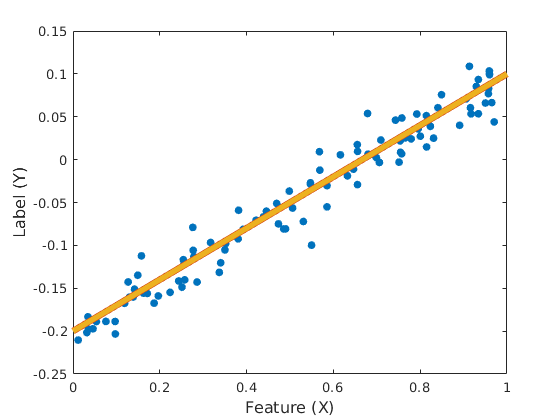
\includegraphics[width=0.8\textwidth]{linear_regression.png}
    \caption{Linear regression for a noisy line.  A blue dot represents the position of a feature/label pair.  The yellow line represents the approximate affine approximation function.}
    \label{fig:linear_regression}
\end{figure}

In the case of unsupervised learning, we are given only some set of features, $\{x\}_{i=1}^N$ and asked to find some pattern in the data.  Finding a patterm can consist of finding clusters of data points which are ``close'' together by some measure, or finding some lower dimensional representation for the data, essentially a problem of lossy compression.  Usually algorithms work by minimizing some loss function so that techniques can be borrowed from supervised learning, though these are not necessarily measures of the algorithm's success.  

One well known example of unsupervised learning is principal component analysis and its cousin singular value decomposition.  Given some features in the form of a matrix $X$, singular value decomposition can find a matrix, $\hat{X}$ of rank $r < rank(X)$ such that $||X-\hat{X}||_F$ is minimzed.  This has the effect of finding a lower dimensional representation of $X$ which contains as much information as possible and therefore tells us which dimensions are ``important.''  One example is shown in figure \ref{fig:svd_recover} uses singular value decomposition to remove noise from an assumed low rank matrix.  In figure \ref{fig:singular_values}, a plot shows the relative contribution of automatically detected signal components.

\begin{figure}
    \centering
    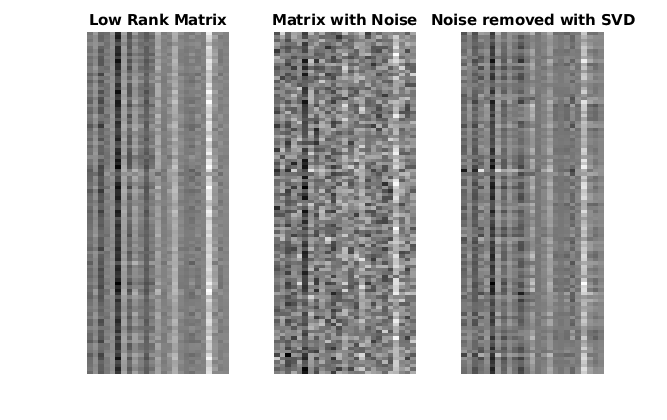
\includegraphics[width=0.8\textwidth]{svd_plots.png}
    \caption{Illustration of using SVD to recover an underlying signal.  This is an example of unsupervsied learning.}
    \label{fig:svd_recover}
\end{figure}
\begin{figure}
    \centering
    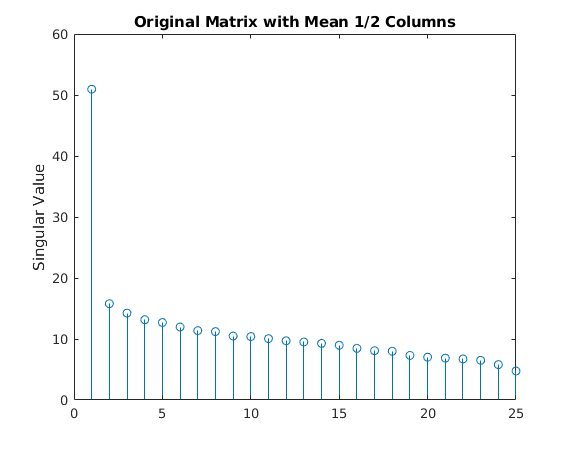
\includegraphics[width=0.8\textwidth]{singval5.png}
    \caption{Set of 25 singular value for the low rank matrix with noise in figure \ref{fig:svd_recover}.  Each column of the original matrix has a mean of about 0.5.  Each singular value is a measure of some signal component present in the matrix.}
    \label{fig:singular_values}
\end{figure}
\begin{figure}
    \centering
    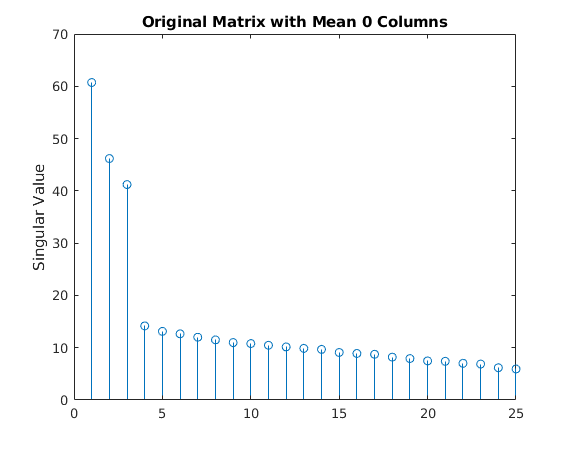
\includegraphics[width=0.8\textwidth]{singval0.png}
    \caption{Set of 25 singular value for a low rank matrix, each column of the original matrix has mean 0.  Here we see three distinct which tells us that the origin rank was very likely three.}
    \label{fig:singval_good}
\end{figure}

\subsection{Hyperparameters} \label{sec:hyperparameters}
Hyperparameters are parameters of a function which do not change during the ``learning process'', that is, they are set by the user at the beginning, and the regular parameters of the function are determined with the hyperparameters held constant.  In the example of using singular value decomposition to denoise a low rank matrix, the hyperparameter would be the desired rank of the resulting matrix.  

We can see from figure \ref{fig:singval_good} that this hyperparameter could be calculated, or at least guessed from the number of dominant singular values.  However, it may be impossible to know what the underlying rank was as in the case of figure \ref{fig:singular_values} if the original matrix does not match our assumptions or if noise dominates the signal.  In most modern machine learning models, it is very difficult to efficiently determine optimal hyperparameters, often requiring a brute force search over several combinations.  This technique is known as grid search, which searches over $n$ hyperparameters on an $n$ dimensional grid and chooses the hyperparameters that minimize some loss function, not neccesarily the same as the model's loss function.  The process of choosing optimal hyperparameters is known as hyperparameter tuning.

\subsection{Overfitting} \label{sec:overfitting}
If we allow our model, or set of permissible functions, to be more complex, we can represent more complicated functions.  Figure \ref{fig:poly_reg} shows an example of both a quadratic fit and a $20^{th}$ order polynomial fit to data points with a more complicated pattern.  These two images represent the issue of overfitting: while the underlying curve is in fact quadratic, the higher order polynomial in fact achieves a lower error.  It is often true, especially in simpler cases, that increasing the model complexity will reduce the error of the objective.  However if our goal is to determine the actual underlying pattern of the data, we may want to choose something simpler.

Regularization is the technique of introducing information to a machine learning problem to reduce overfitting.  One of the most common forms of regularization is called Tikhanov regularization.  It is also known by the names of ridge regression in statistics and weight decay in machine learning.  In linear regression, Tikhanov regularization penalizes a function according to the magnitude squared of each coefficient.  By the Riesz representation theorem, for any linear function, $f: \mathbb{R}^m \rightarrow \mathbb{R}$, $\exists v\in\mathbb{R}^m \text{ s.t. } f(x) = \langle x,v\rangle $ for some vector $v\in \mathbb{R}^m$.  Suppose $v$ is the vector corresponding to linear function $g$ in this manner, then for linear regression the new loss function is given in equation \ref{eq:tik}
\begin{align}\label{eq:tik}
L(g,x,y) = ||g(x_i)-y_i||^2 + \lambda ||v||_2^2
\end{align}
where $\lambda$ is a real scalar hyperparameter that may be tuned in the manner discussed in section \ref{sec:overfitting}.  While there is no efficient method for computing the optimal value for $\lambda$ in general, it has a simple value given a certain assumption.  If we assume a Gaussian distribution with 0-mean and $\lambda^{-1}$ variance for the prior distribution of the vector $v$, then the result of the maximum a posteriori (MAP) estimation is the same as the solution to equation \ref{eq:tik}.

\begin{figure}
    \centering
    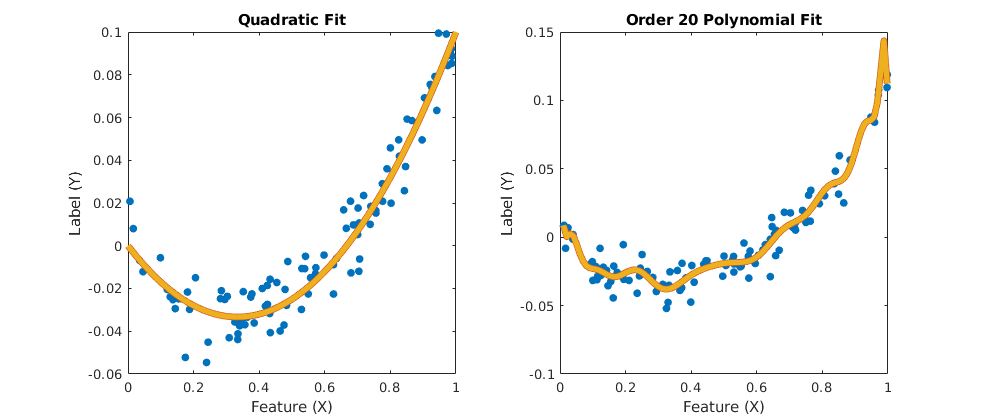
\includegraphics[width=\textwidth]{overfitting.png}
    \caption{The figure on the left is the result of an optimization constrained to second order polynomials while the figure on the right is the result of a $20^{th}$ order constraint.  The second order constraint achieves a result closer to the underlying curve.}
    \label{fig:poly_reg}
\end{figure}

\subsection{Training, Validation, and Testing}
Using the loss function over all data points is not a suitable measure of the success of a machine learning algorithm.  As we discussed in section \ref{sec:overfitting}, models which fit the underlying function worse may easily achieve a better overall loss.  In fact for any finite dataset that could feasible represent a function, it is easy to find a function in the form of a hash table that can exactly represent the mapping of inputs to outputs.  Of course, this hash table would not ``generalize'' to other data points and wouldn't represent the underlying function in a meaningful way.  

To help mitigate this issue, it is standard to separate the data into three parts: training, validation, and testing.  Essentially, training is used to tune regular parameters, validation is used to tune hyperparameters, and testing is used only to evaluate the effectiveness of the algorithm.
